\subsection{Anatomy}
The prostate is an organ in the human male body located in the pelvis, under the bladder, and in front of the rectum. It is a small, walnut-sized gland that surrounds the urethra, a tube that expels urine from the human body. The prostate is responsible for producing the seminal fluid that creates semen when mixed with sperm produced by the tescticles.
Due to its proximity to vital structures such as the bladder and rectum, the prostate is a crucial part of the male reproductive system. Monitoring prostate health is essential because issues such as prostate enlargement or prostate cancer are common in older men, often necessitating precise imaging for accurate diagnosis and treatment planning.
\begin{figure}[h]
\centering
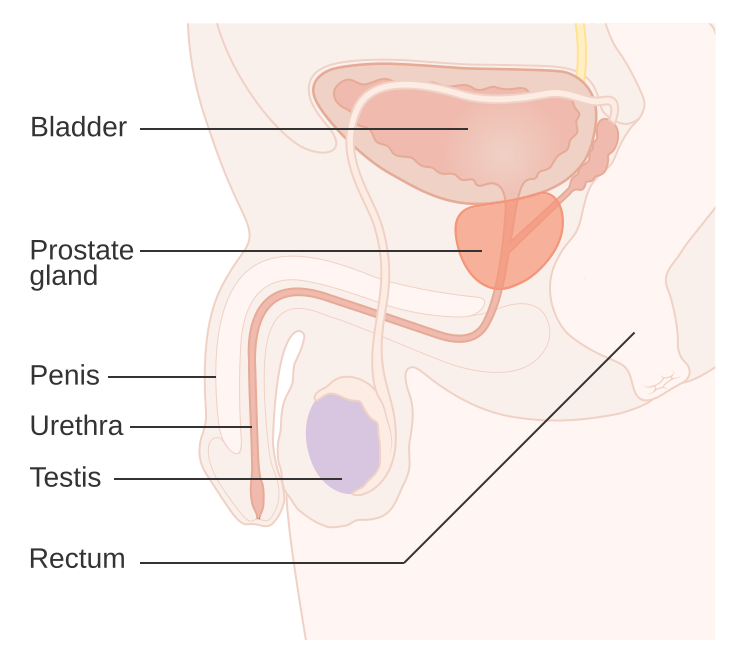
\includegraphics[width=0.7\textwidth]{background/Diagram_showing_the_position_of_the_prostate_and_rectum_CRUK_358.svg.png}
\caption{Visualization showing where a prostate is located\cite{prostate-rectum-image}.}
\end{figure}

\newpage
\subsection{Prostate cancer}
Prostate cancer is a tumour that grows in the prostate. During growth, it can press against the urethra, triggering the symptoms described below.
Cancer can spread to other organs of the body, so it is important to detect the disease early and monitor it properly. 
The 5-year survival rate for one with the condition is between 30-99 percent.

This cancer ranks as the world's second most common cancer among men, after lung cancer. In 2020, there were approximately 1.4 million diagnosed cases and 375,000 deaths worldwide\cite{culp_recent_2020}.
In Europe, it is the most commonly diagnosed cancer in males and the third leading cause of cancer-related deaths, what can be observed in Poland (Fig. [\ref{fig:prostate-cancer-occurences}]). 

\begin{figure}[H]
\begin{subfigure}[b]{0.5\textwidth}
    \centering
    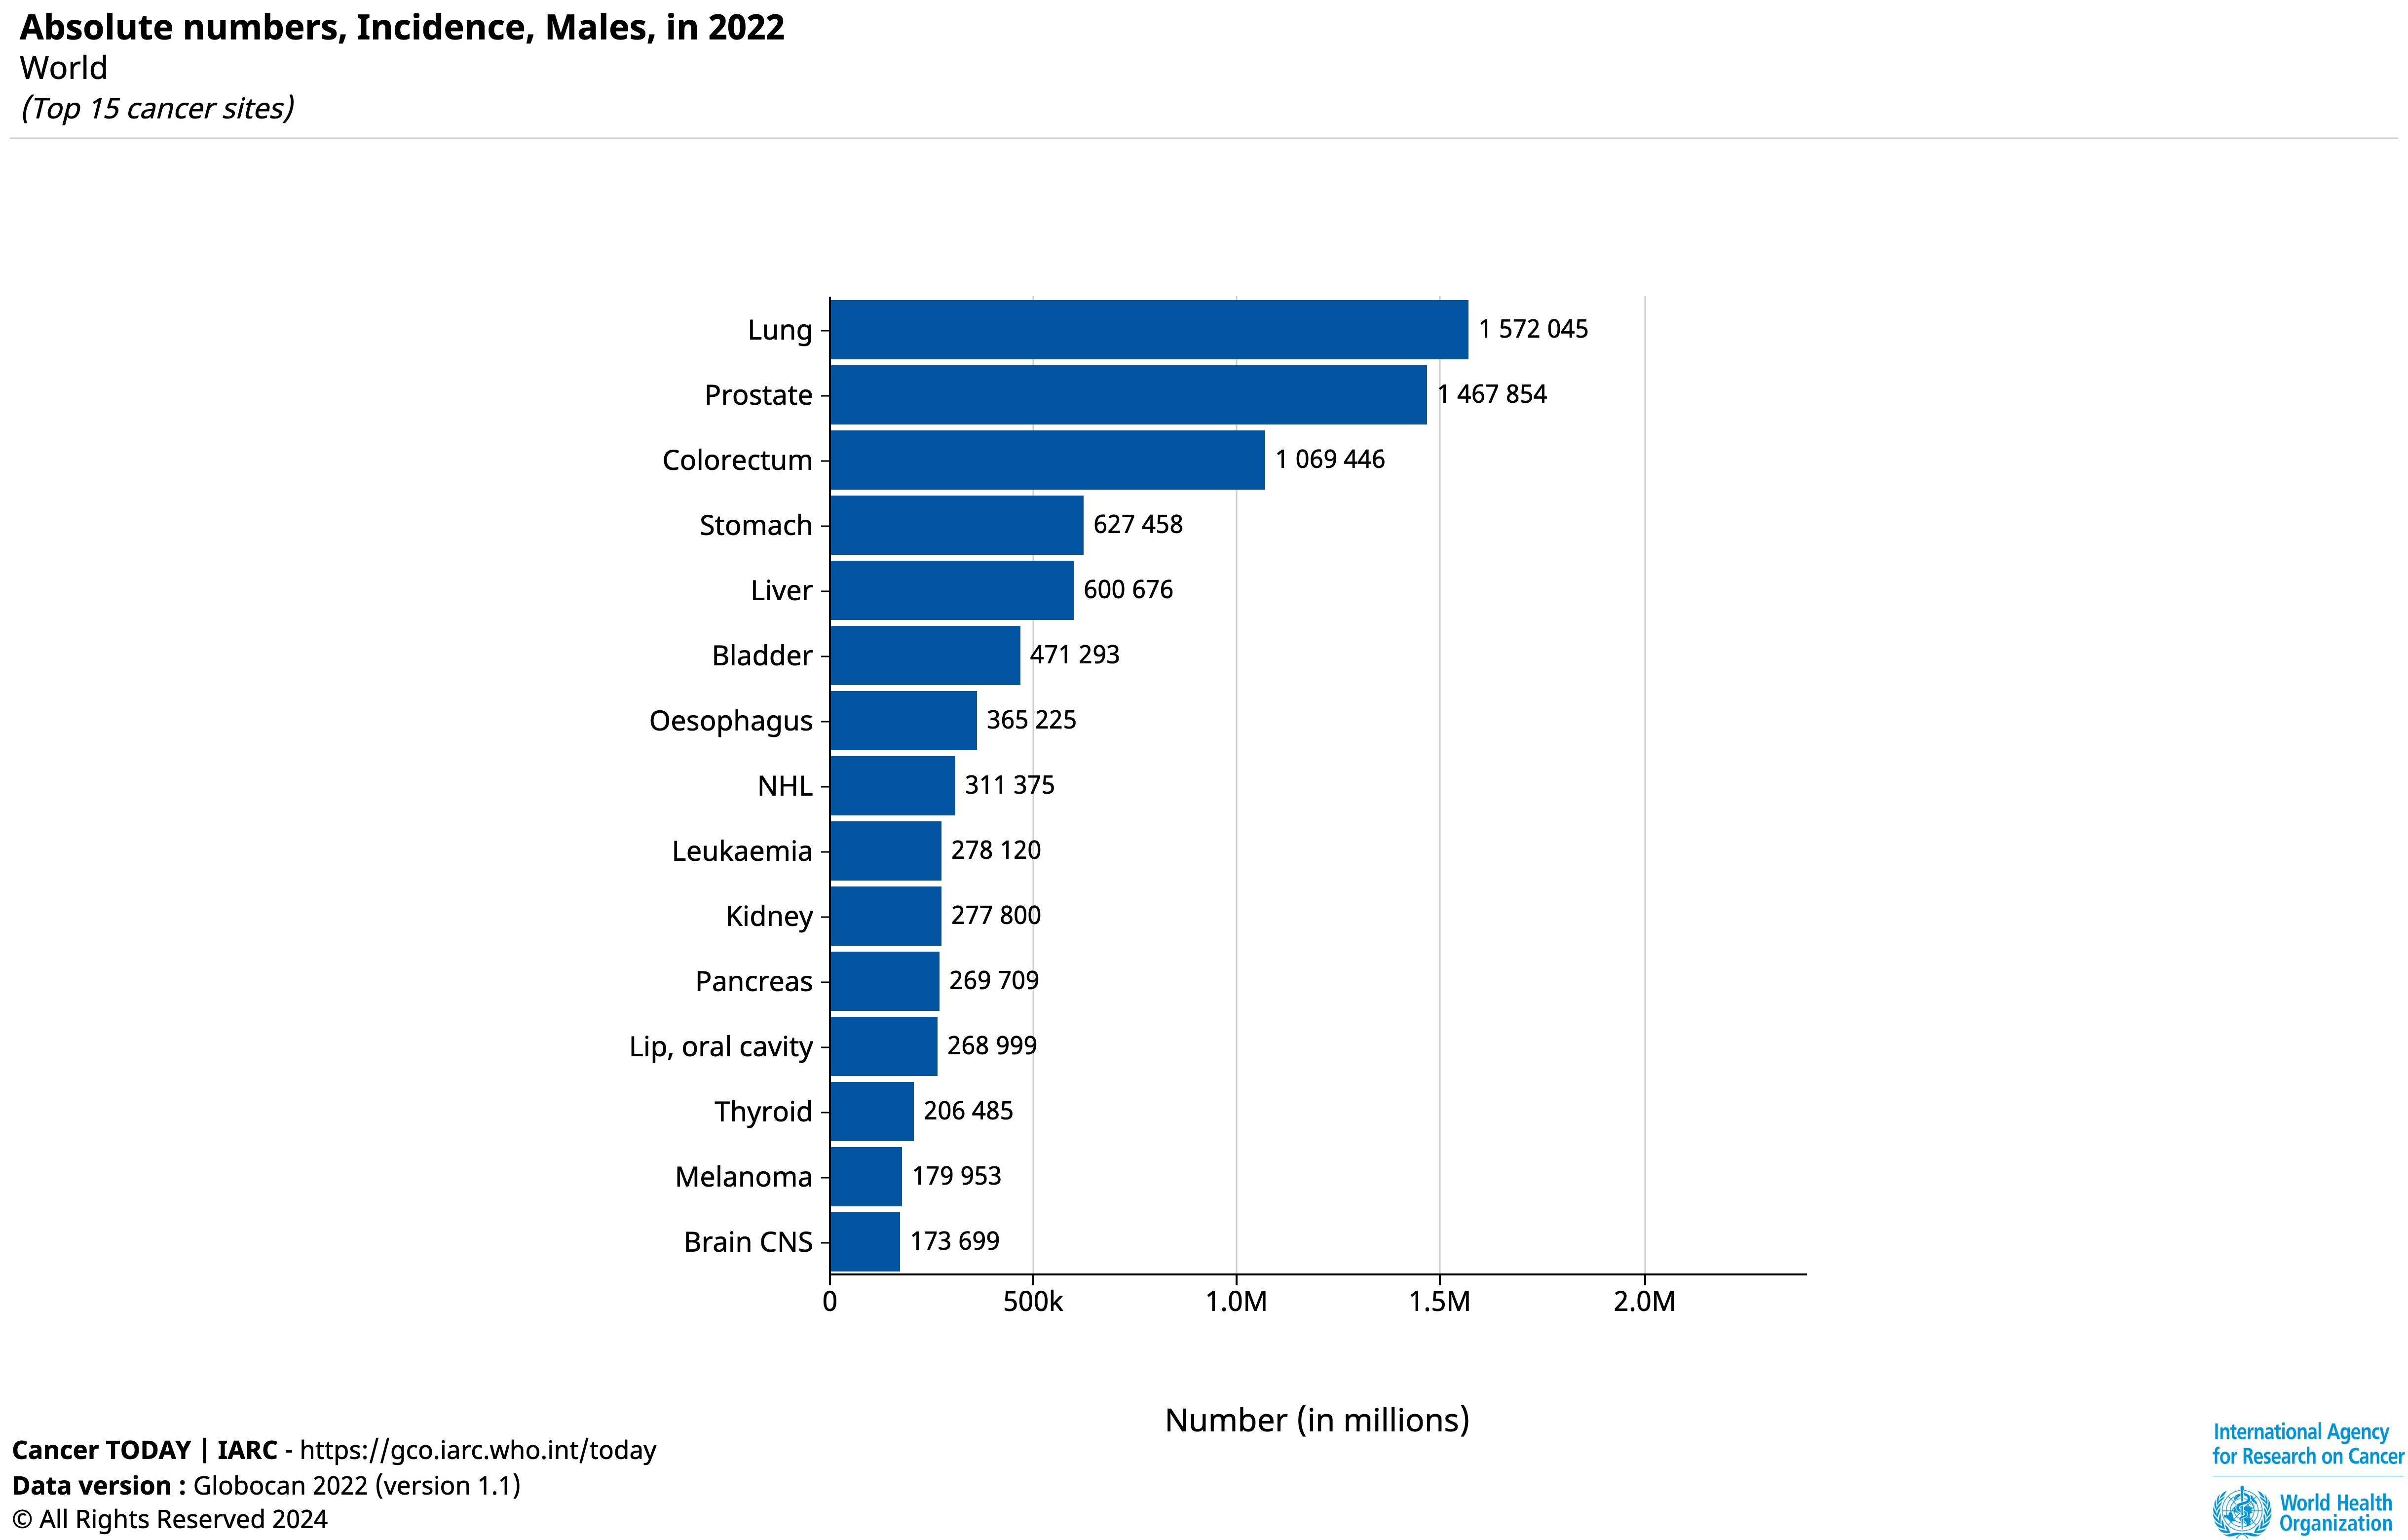
\includegraphics[width=1\linewidth]{background/graphic-absolute-numbers-inc-males-in-2022-world.png}
    \label{fig:pc-incidence-world}
\end{subfigure}
\begin{subfigure}[b]{0.5\textwidth}
    \centering
    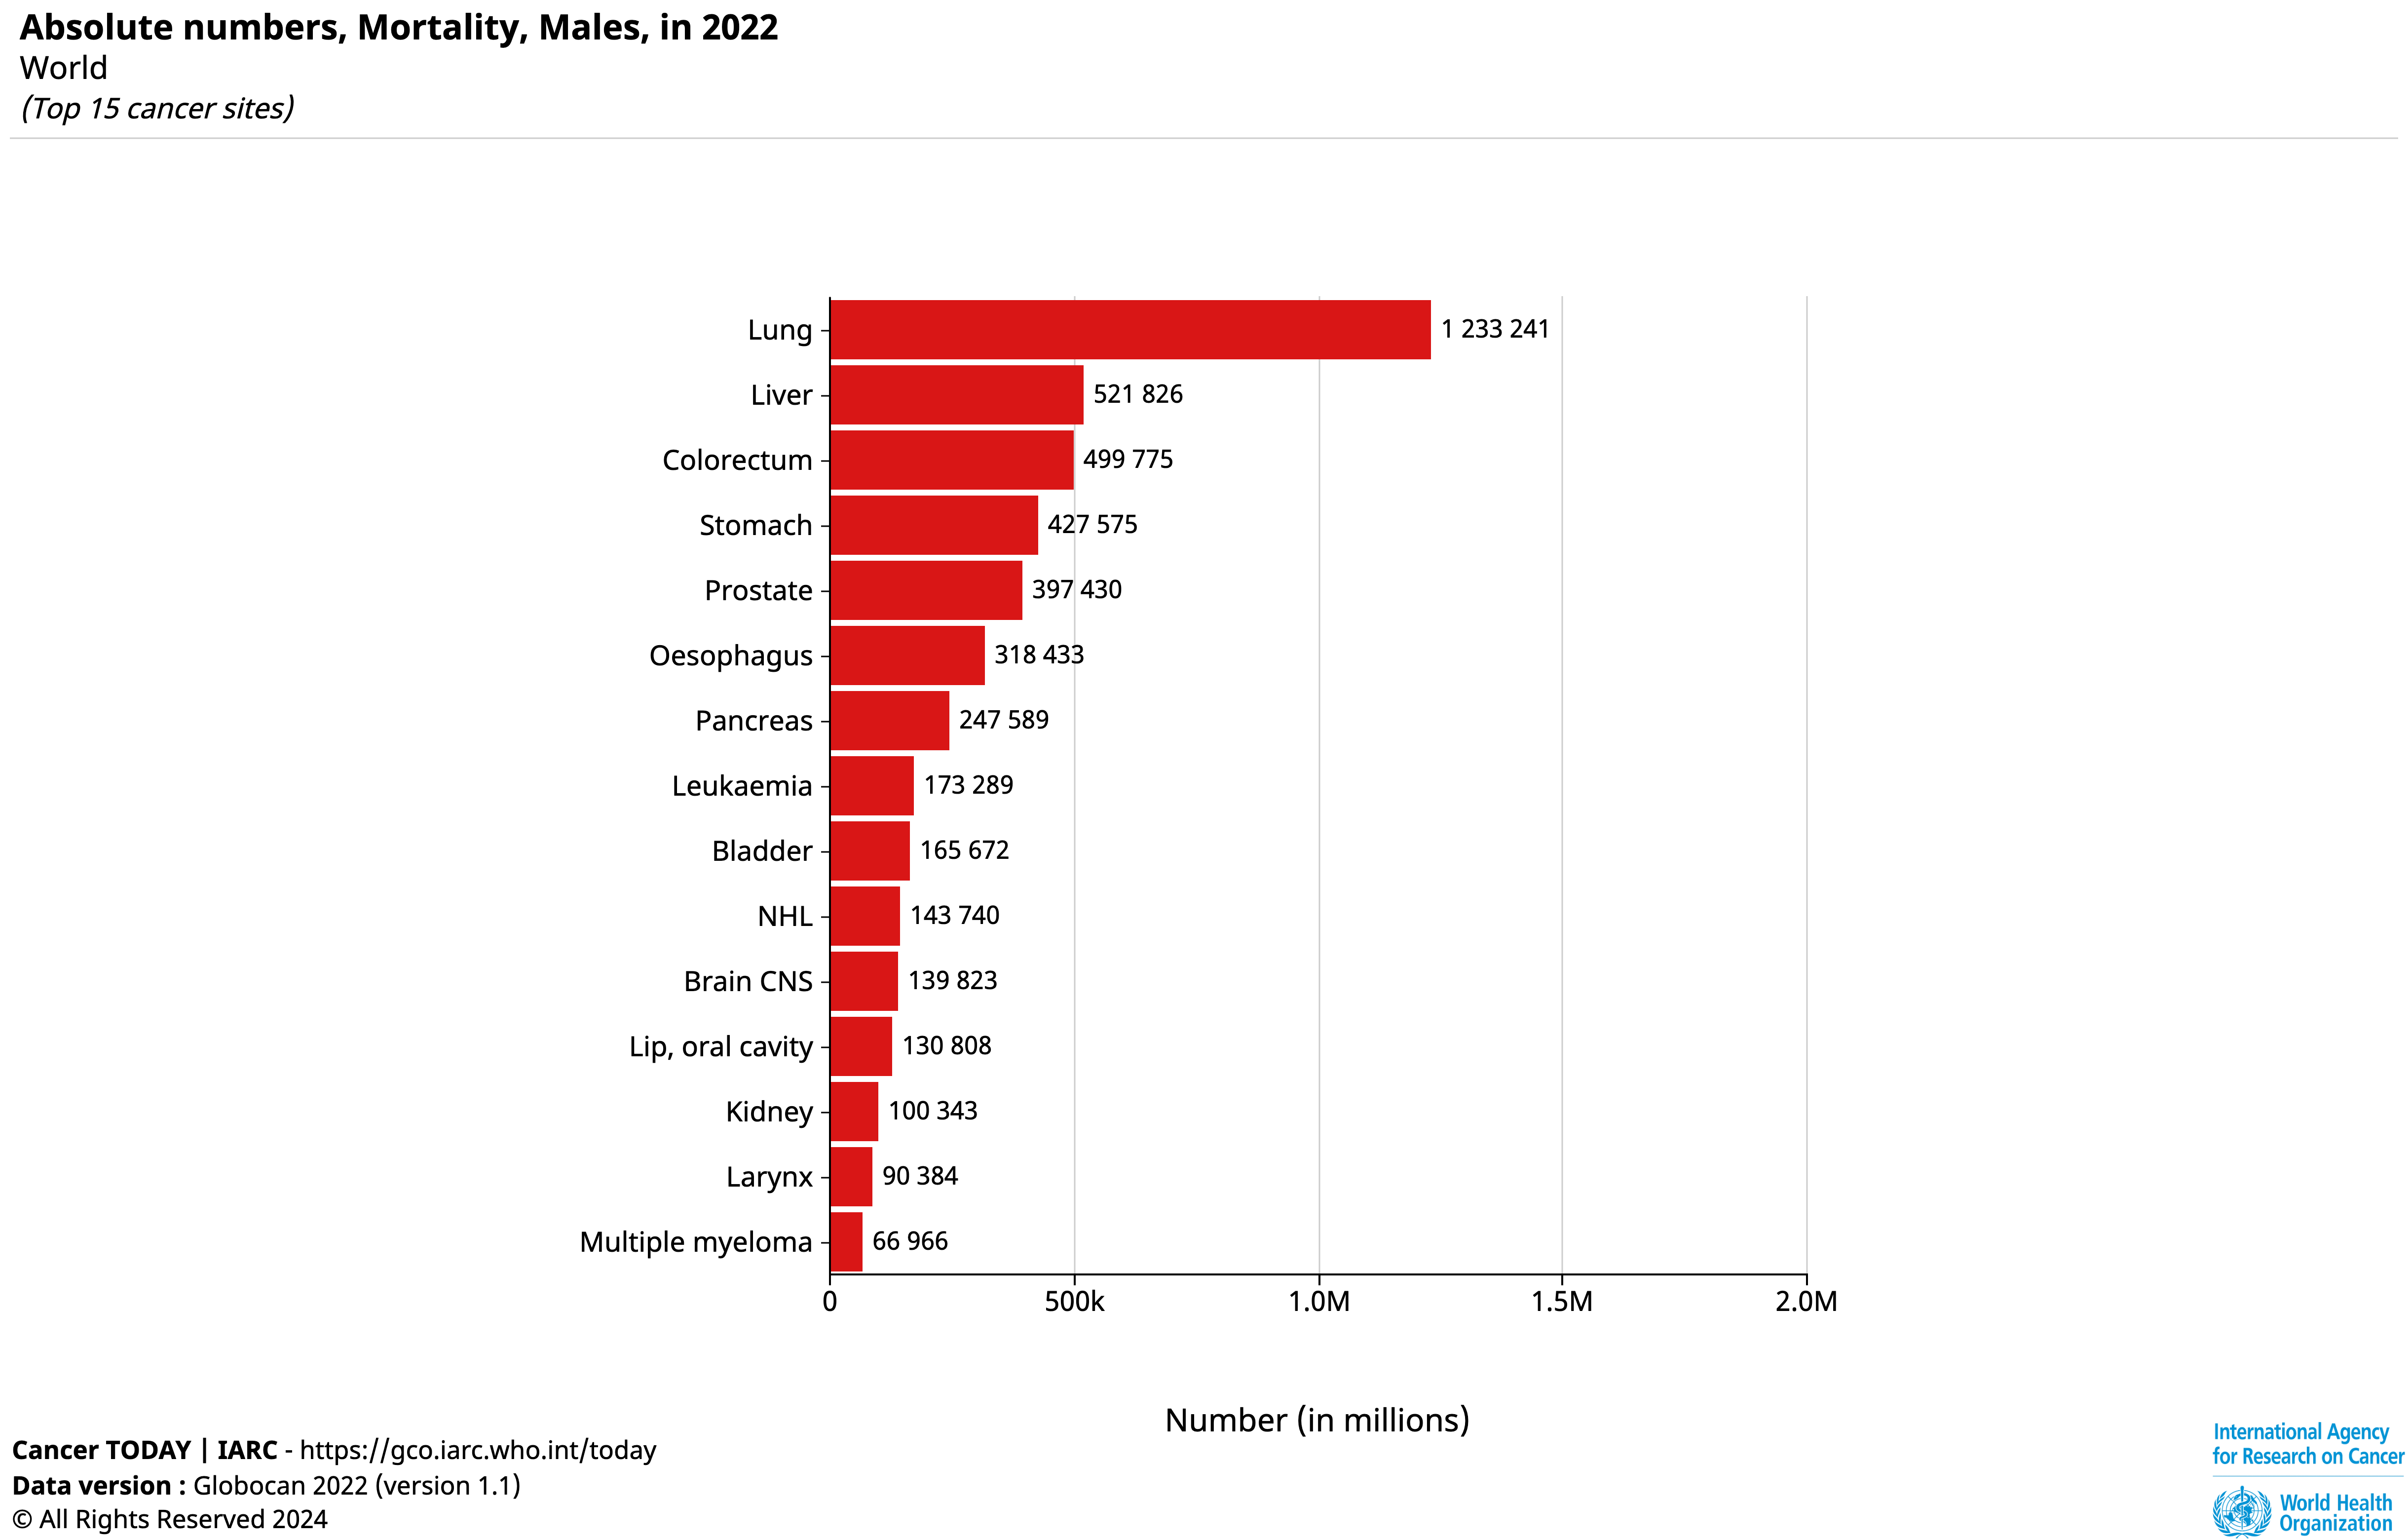
\includegraphics[width=1\linewidth]{background/graphic-absolute-numbers-mort-males-in-2022-world.png}
    \label{fig:pc-mortality-world}
\end{subfigure}
\caption{Absolute numbers of prostate cancer incidence and mortality in males in the world in 2022.\cite{gco_cancer_today}.}
\end{figure}

\begin{figure}[H]
    \centering
    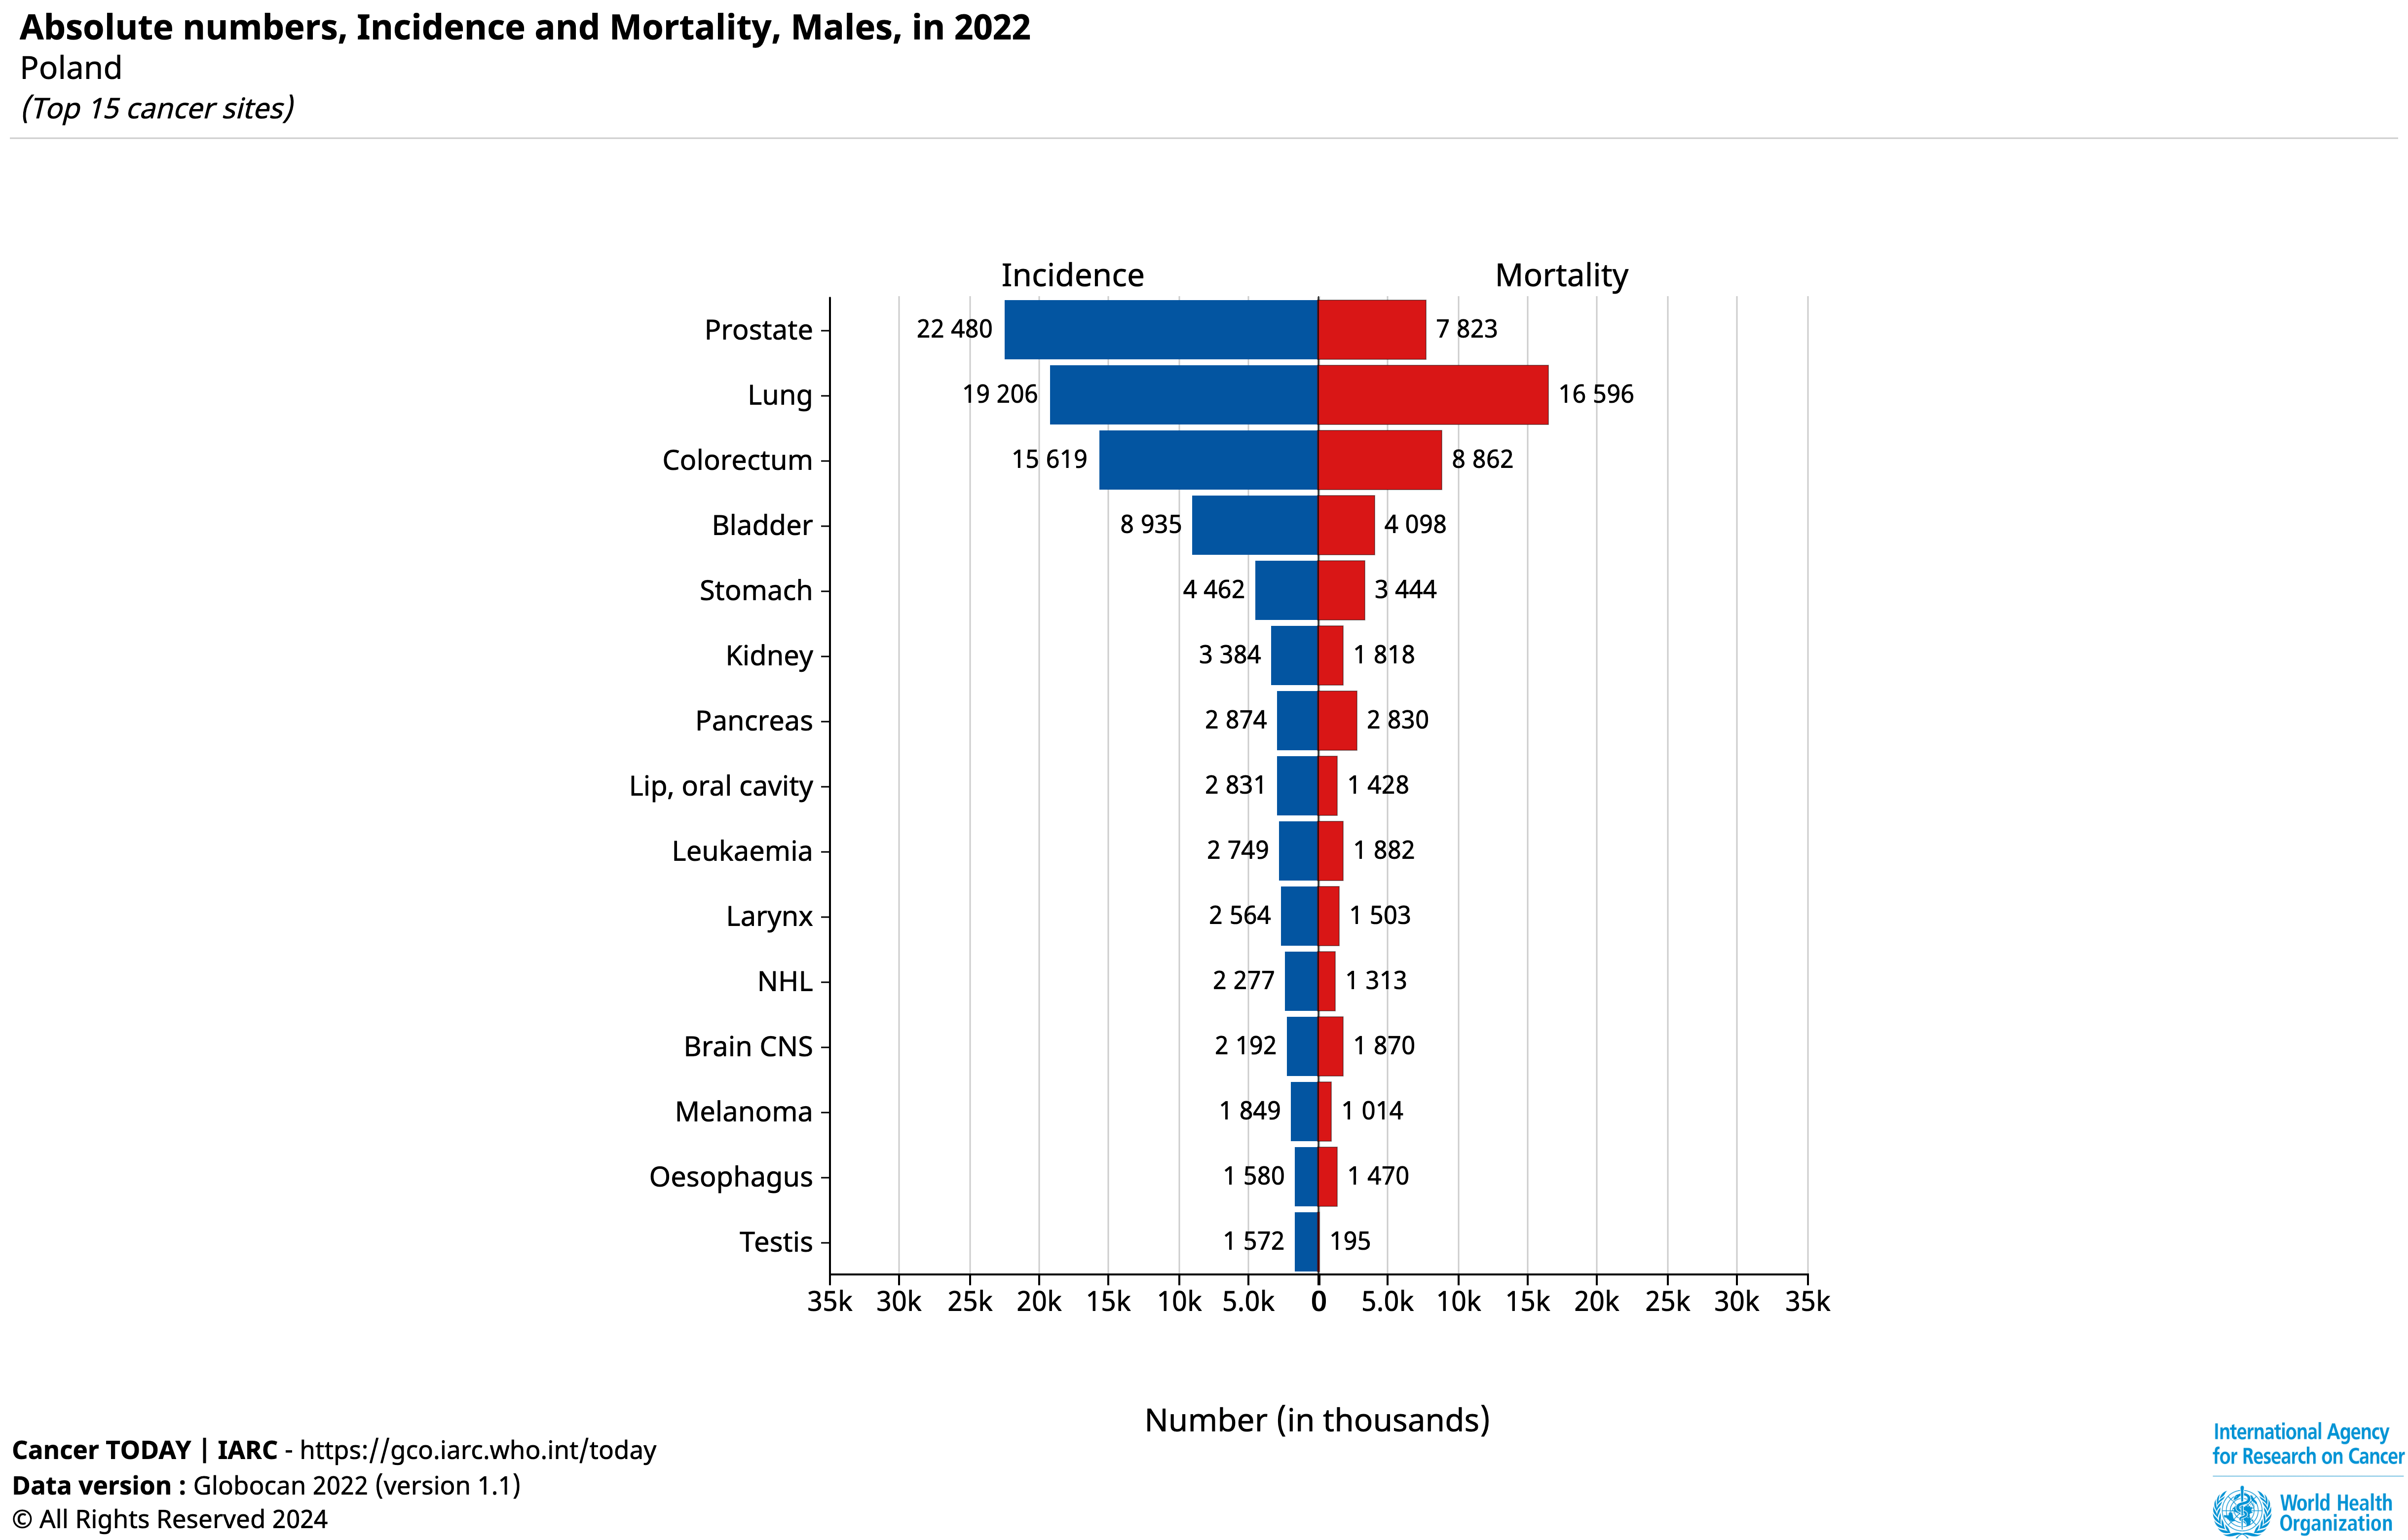
\includegraphics[width=0.5\linewidth]{background/graphic-absolute-numbers-inc-and-mort-males-in-2022-poland.png}
    \caption{Absolute numbers of prostate cancer incidence and mortality in males in Poland in 2022\cite{gco_cancer_today}}.
    \label{fig:prostate-cancer-occurences}
\end{figure}

Chris Parker, Prostate cancer specialist at the Institute of Cancer Research in the United Kingdom, says that even 80 percent of old men have prostate cancer, but they are never diagnosed with it\cite{nhs_choices_2024}. 


\begin{figure}[H]
    \centering
    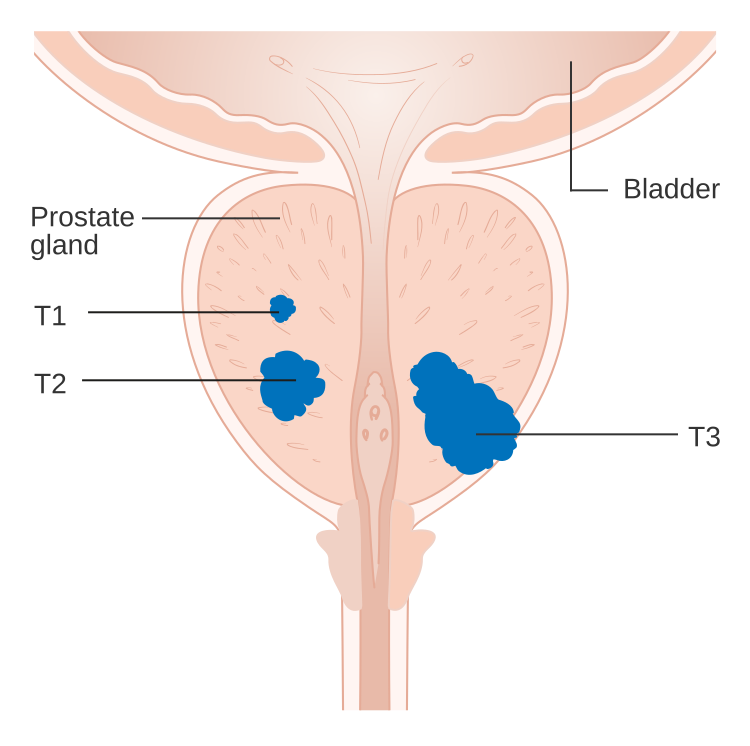
\includegraphics[width=0.5\linewidth]{background/Diagram_showing_T1-3_stages_of_prostate_cancer_CRUK_278.svg.png}
    \caption{Three stages of prostate cancer\cite{pc-stages}.}
    \label{fig:prostate-cancer-stages}
\end{figure}

\paragraph{Symptomps}\mbox{} \\

Prostate cancer can lead to\cite{prostate-cancer-symptomsandcauses_2024}\cite{nhs_choices_2024}:
\begin{itemize}
    \item troubles with urinating,
    \item blood in the urine,
    \item blood in the semen,
    \item bone pain,
    \item weight loose,
    \item erectile dysfunction,
    \item need to use toilet more frequently,
    \item need to use toilet more urgently.
\end{itemize}

\paragraph{Causes\cite{nhs_choices_2024}}\mbox{} \\
\indent Causes of prostate cancer of prostate cancer are not known. However, there are certain things that increase the risk of having the condition. 
Most cases of prostate cancer are diagnosed in men aged 50 or older. 
Men whose relatives were affected by the condition have a slightly increased risk of having it. Recent research suggests that obesity could have an influence on the risk of prostate cancer.

\paragraph{Diagnosis\cite{nhs_choices_2024}}\mbox{} \\
There are multiple tests that can help detect prostate cancer. 
Most commonly used tests are\cite{nhs_choices_2024}:
\begin{itemize}
    \item blood tests - Prostate-specific antigen (PSA) test, it measures the level of PSA in the blod; the test can help detect cancer in an early stage.
    \item physical examination,
    \item biopsy,
    \item medical imaging - MRI and CT scans.
\end{itemize}

\paragraph{Treating prostate cancer\cite{nhs_choices_2024}}
\begin{itemize}
    \item active surveillance,
    \item surigical removal of the prostate,
    \item radiation therapy,
    \item hormone therapy,
    \item chemotherapy.
    
\end{itemize}

% \newpage
\subsection{Medical imaging}
Medical imaging is the technique and process used to produce visual representations of the interior of a body for clinical evaluation and medical treatment. It enables doctors to examine the structures of the body, diagnose illnesses, direct treatments and track the progress of diseases. Various methods of medical imaging exist, each crafted to emphasize different aspects of the body's health. The main ones are the following.

\begin{itemize}
    \item Computed Tomography (CT),
    \item Magnetic Resonance Imaging (MRI),
    \item Ultrasound (USG),
    \item Positron Emission Tomography (PET).
\end{itemize}

\begin{figure}[H]
    \centering
    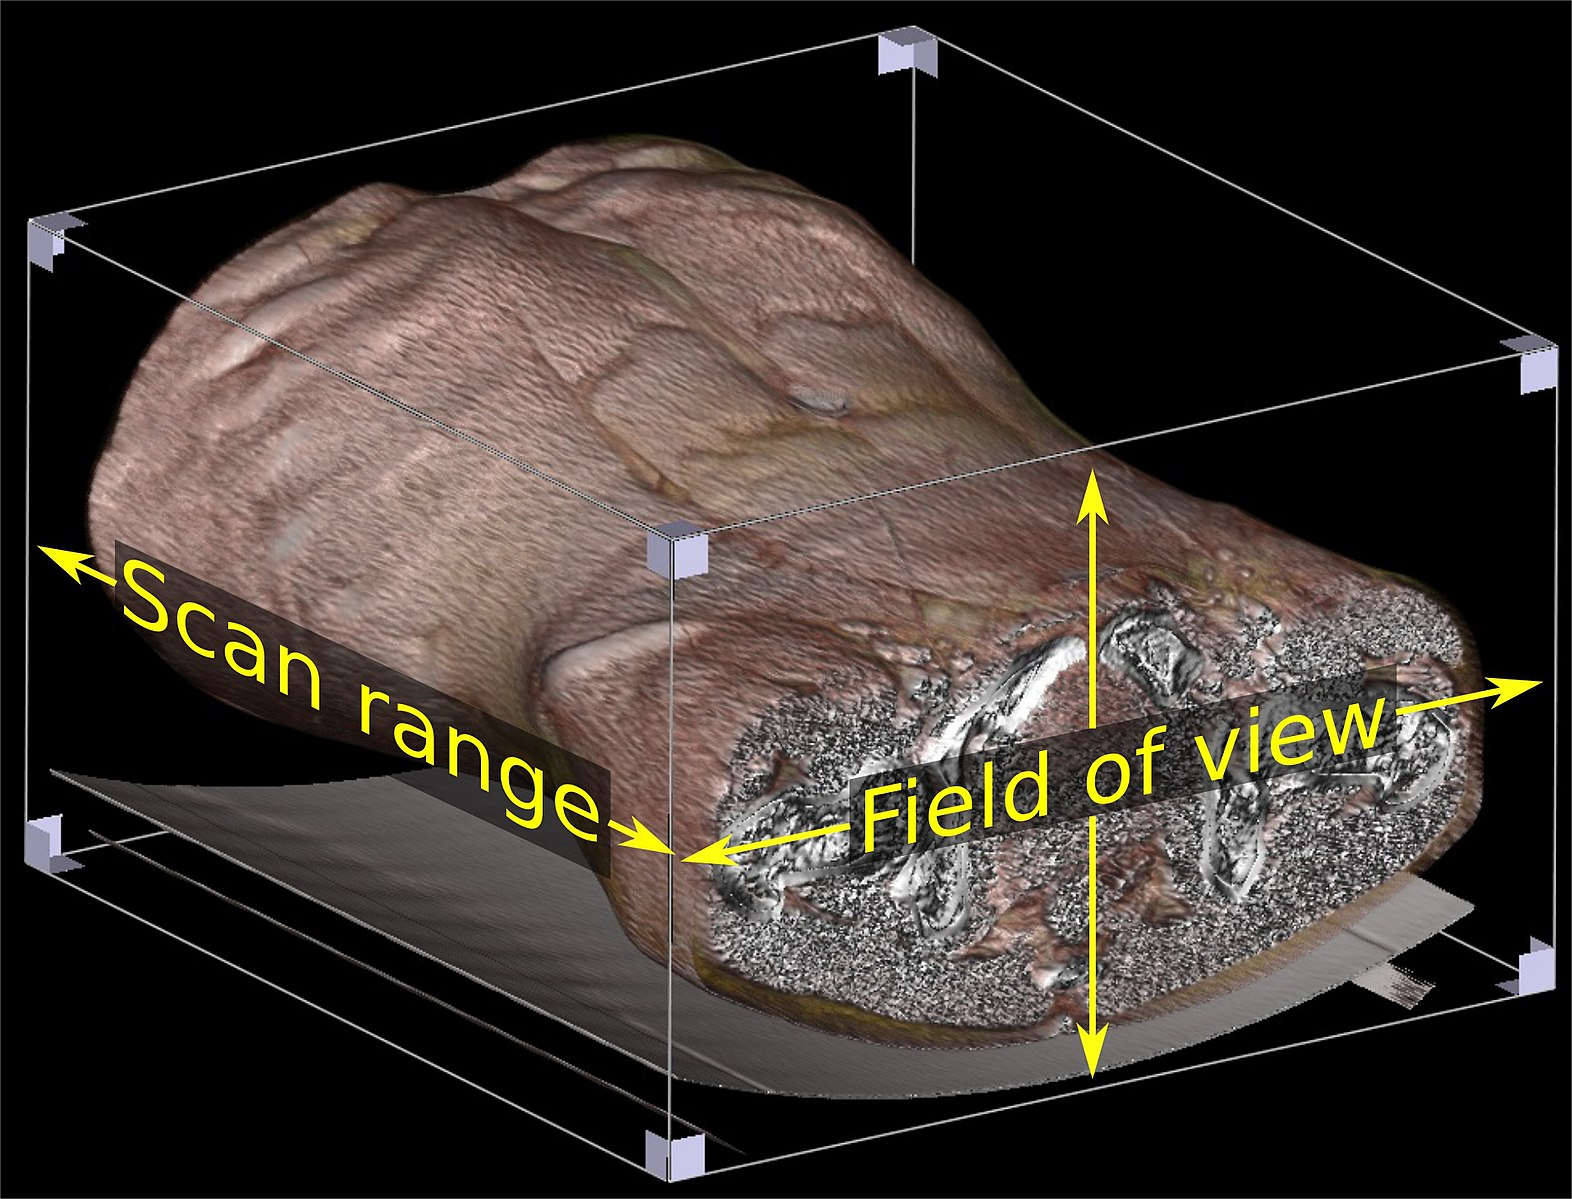
\includegraphics[width=0.5\linewidth]{background/1572px-Abdominal_CT_with_scan_range_and_field_of_view,_with_box_and_text.jpg}
    \caption{Abdominal CT scan\cite{abdominal-ct-scan}.}
    \label{fig:ct-scan-abdominal}
\end{figure}

In this study, our emphasis will be on computed tomography, as the dataset we are using was generated through this method. However, datasets acquired through other approaches could be similarly expanded using the deep learning techniques described later.

% \subsubsection{MRI- Magnetic resonance imaging}

% \begin{figure}[H]
%     \centering
%     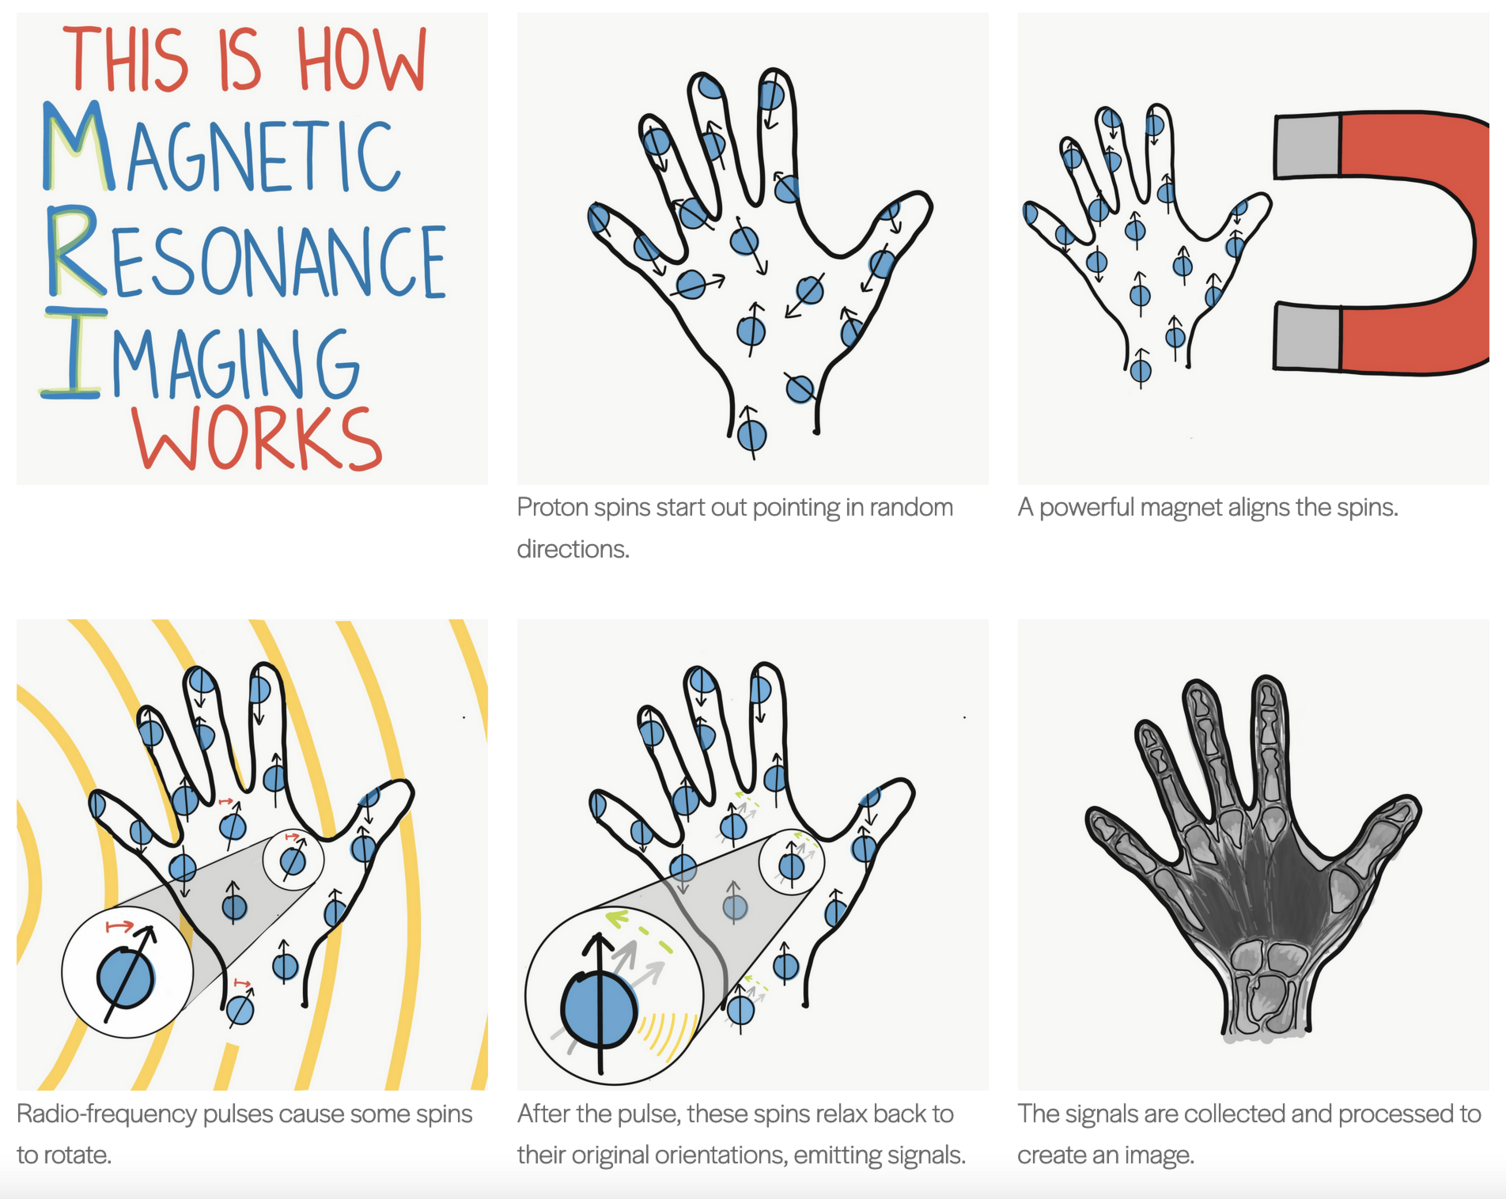
\includegraphics[width=0.99\linewidth]{background/Magnetic_Resonance_Imaging.png}
%     \caption{Explanation how magnetic resonance imaging (MRI) works\cite{mri-scan-how-it-works}.}
%     \label{fig:enter-label}
% \end{figure}

\newpage
\subsubsection{CT - Computed Tompography}
Computed tomography (CT) is a medical imaging technique that produces detailed cross-sectional images of the body. The word "tomography" comes from Ancient Greek, where "tomos" means "to slice" and "graphō" means "to write". 

The slicing of the human body is achieved using X-rays and advanced computer algorithms. Unlike conventional X-rays, which produce flat, two-dimensional images, CT scans produce 3D images by combining multiple X-ray measurements taken from different angles around the body. 

During a CT scan, an X-ray source rotates around the patient. Meanwhile, detectors on the opposite side capture the X-rays as they pass through the body. The X-rays are weakened as they pass through different tissues, such as bone, muscle and fat, which absorb different amounts of radiation. This rotating X-ray system produces multiple images or 'slices' of the body, typically only a few millimetres thick. A computer then processes these images to produce detailed cross-sectional images of the inside of the body. These multiple slices can be combined to create a 3D representation of the area being examined. 

% \begin{figure}[H]
%     \centering
%     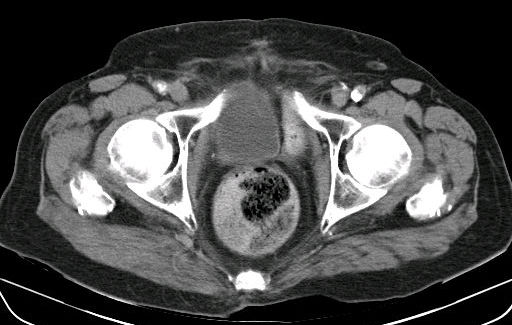
\includegraphics[width=0.5\linewidth]{background/ImpacFecal_149.jpg}
%     \caption{One slice of a tompography scan of prostate and pelvis\cite{ct-scan-prostate}.}
%     \label{fig:enter-label}
% \end{figure}
% - DICOM format for saving CT data.

\begin{figure}[H]
    \centering
    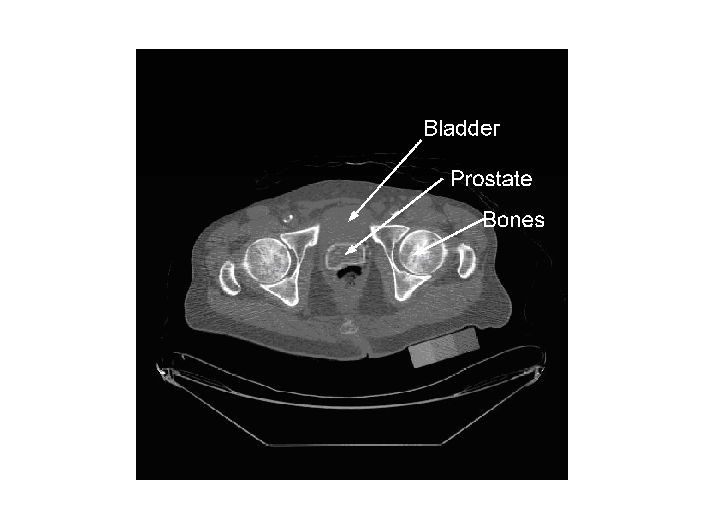
\includegraphics[width=0.9\linewidth]{background/A-typical-2-D-pelvic-CT-scan-Left-Manually-segmented-prostate-region-marked-by-a.png}
    \caption{Single layer from a 3-D pelvic CT scan. Segmented manually and marked by a radiologist\cite{inproceedings}.}
    \label{fig:enter-label}
\end{figure}

\newpage
\subsection{Cancer detection}
% Prostae cancer is usually detected using blood tests. Medicians do not use CT scans to diagnose the condition. They are used to check whether prostate cancer has spread to other parts of the body. 
Prostate cancer is detected by a combination of diagnostic tests, starting with a PSA (prostate specific antigen) blood test and a digital rectal examination. If abnormalities are found, a biopsy is often carried out to confirm the presence of cancer cells. Once diagnosed, imaging tests such as CT (computed tomography) scans are essential for staging the cancer, especially in advanced stages. CT scans can show whether the cancer has spread to other areas, such as lymph nodes, bones or distant organs. This information is crucial in determining the most effective treatment approach, including surgery, radiotherapy or systemic therapies.
\paragraph{Cancer detection using Artificial Intelligence}\mbox{}\\
\indent In the case of prostate cancer, AI is primarily used for segmentation rather than initial detection. Detection is typically done by other diagnostic means. Once prostate cancer is identified, AI plays a crucial role in analyzing medical imaging data, particularly CT scans. AI-powered segmentation algorithms, for example U-Nets, can precisely mark the boundaries of the prostate gland, tumor, and surrounding tissues in these scans. This accurate segmentation is essential for treatment planning. Determining the exact location and extent of a tumour can be the basis for targeted radiotherapy or surgery. AI can also help monitor treatment. It can aid track the cancer progress and detect subtle changes in tumour size or shape over time. While AI improves the accuracy and efficiency of image analysis, it is important to note that it is a tool to assist healthcare professionals rather than a stand-alone diagnostic method. 

\paragraph{Limitations}\mbox{}\\
\indent One of the limitations of using AI in this context is the need for large and diverse datasets to train such models. Unfortunately, the medical imaging field suffers from training data insufficiency caused by data privacy, lack of standardized ways of collecting such data by multiple institutions, and throughput of CT scanners. 
This problem raised the idea of using data augmentation techniques in order to enlarge already existing datasets and it formed the basis for the subject of this thesis.
% \paragraph{State of the art techniques for cancer detection}

\newpage
\subsection{Data augmentation}
Data augmentation is a technique for enlarging existing dataset with new samples created from already existing ones. There exist many techniques that allow us to do so. The more traditional ones focus on transformations of the original images. However, with the rise of artificial intelligence, generative techniques have emerged that allow us to generate artificial samples using deep learning models. In this work, we will focus on generative models that can create synthetic samples from Gaussian noise. 

% \begin{figure}[H]
%     \centering
%     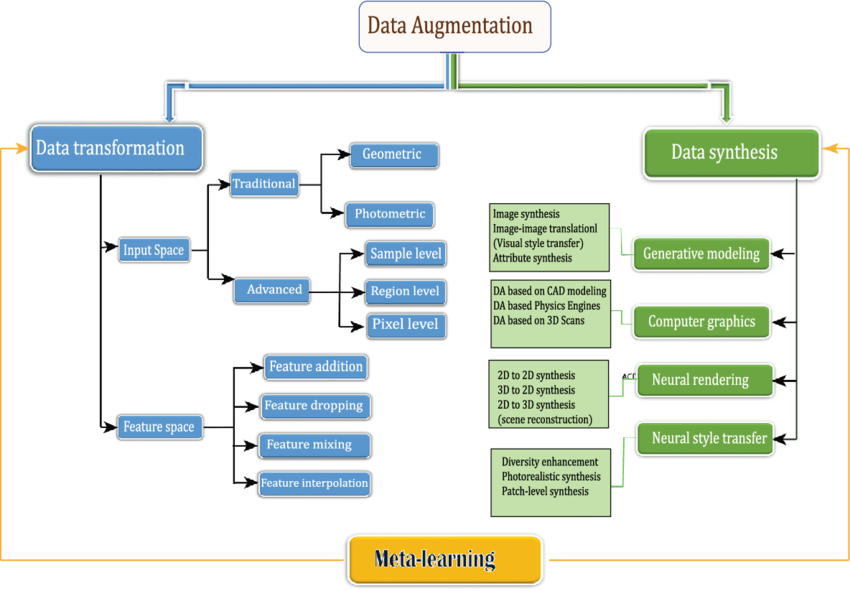
\includegraphics[width=0.99\linewidth]{background/Taxonomy-of-data-augmentation-approaches-used-in-this-survey.png}
%     \caption{Data augmentation taxonomy\cite{Mumuni2022-ka}.}
%     \label{fig:enter-label}
% \end{figure}

\begin{figure}[H]
    \centering
    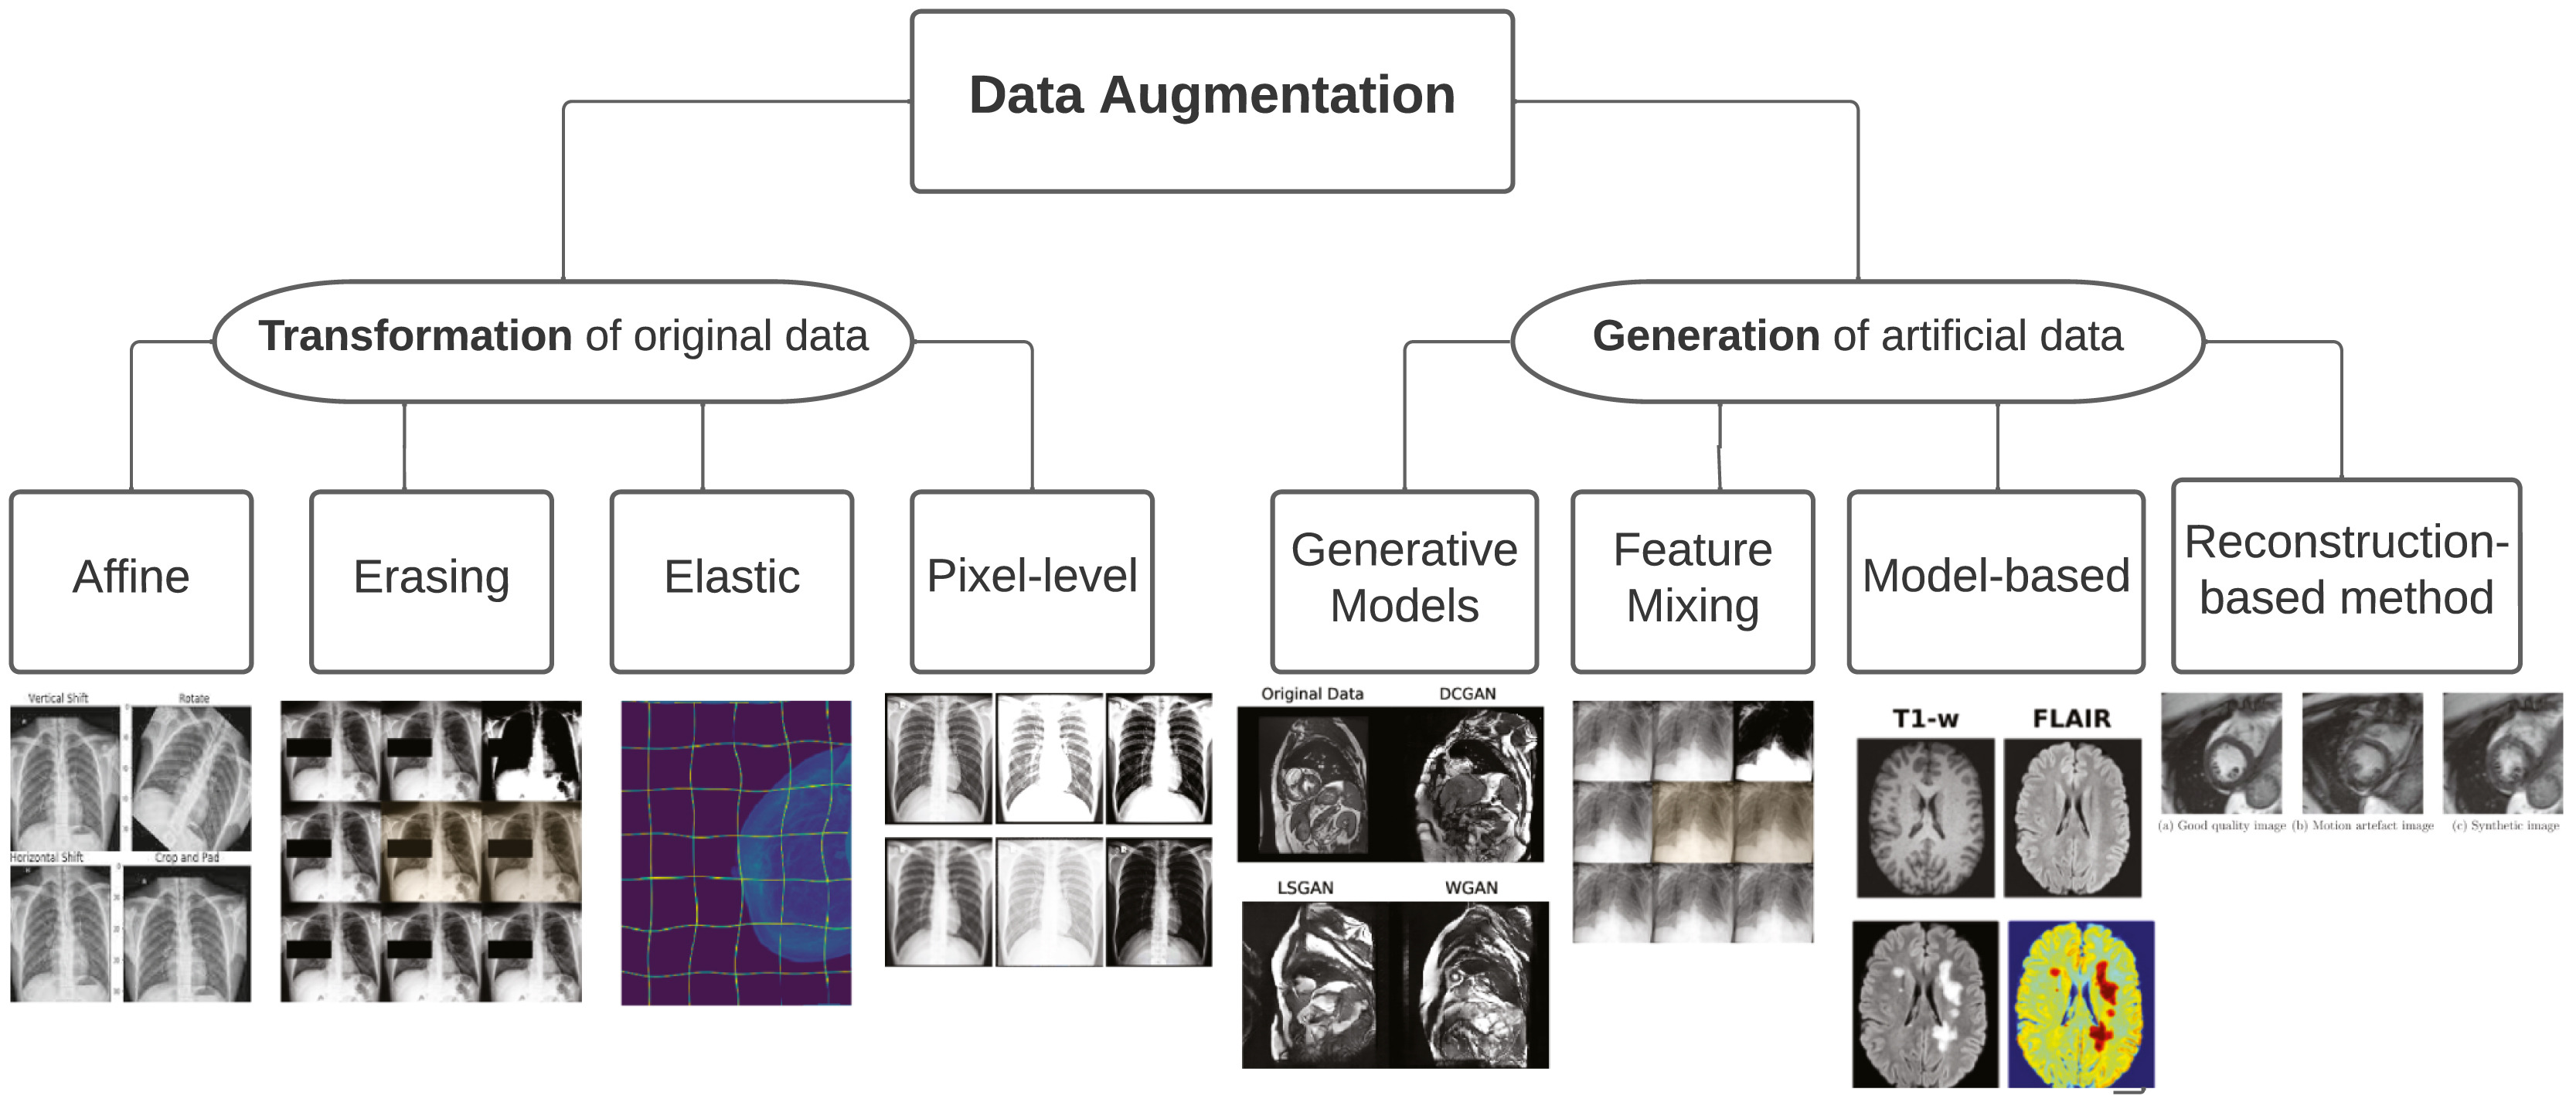
\includegraphics[width=0.99\linewidth]{background/taxonomy-data-augmentation.jpg}
    \caption{Data augmentation taxonomy\cite{GARCEA2023106391}.}
    \label{fig:enter-label}
\end{figure}

% The types of transformations
% \paragraph{Affine transformations} are geometric transformations that preserve lines and parallelism. They do not preserve angles and distances. Exemplary are: rotating, translating, scaling, horizontal and vertical shifting, cropping, padding, shearing.

% \paragraph{Erasing transformation} are used to replace some part of an image with some fixed value or random noise. 

% \paragraph{Pixel level}



\subsection{Generative Medical Imaging}
Medical imaging field in the AI landscape suffers from insufficient data. Thus scientists around the world started to explore generative networks. Now they are the most popular solution for the generation of medical images\cite{osuala2023data}.
Generative models provide a greater potential for data augmentation, in comparison to transformation techniques, by producing a wider variety of samples. However, these methods are much more complex and require significant computational resources.

Artificial samples obtained this way may not have the same visual characteristics or distribution as the original set. Additionally, the samples obtained in this way may include artifacts, even invisible to the human eye, that could be harmful to the models that would be trained on them.
\subsection{State of the art techniques for generative medical imaging}